\documentclass[journal]{IEEEtran}
\usepackage{cite}
\usepackage[pdftex]{graphicx}
\graphicspath{{./images/}}
% *** MATH PACKAGES ***
\usepackage[cmex10]{amsmath}
% *** SPECIALIZED LIST PACKAGES ***
\usepackage{algorithmic}
% *** ALIGNMENT PACKAGES ***
\usepackage{array}
%\usepackage{mdwmath}
%\usepackage{mdwtab}
%\usepackage{eqparbox}
% *** SUBFIGURE PACKAGES ***
%\usepackage[tight,footnotesize]{subfigure}
%\usepackage[caption=false]{caption}
%\usepackage[font=footnotesize]{subfig}
% *** FLOAT PACKAGES ***
%\usepackage{fixltx2e}
\usepackage{stfloats}
% *** PDF, URL AND HYPERLINK PACKAGES ***
%\usepackage{url}
% \url{my_url_here}.
% *** Do not adjust lengths that control margins, column widths, etc. ***
% *** Do not use packages that alter fonts (such as pslatex).         ***

% correct bad hyphenation here
\hyphenation{op-tical net-works semi-conduc-tor}

\begin{document}
%
% paper title
% can use linebreaks \\ within to get better formatting as desired
\title{Toward Real-Time State Estimation and Tracking of Elastic Rods}
\author{Bardia~Mojra}
% make the title area
\maketitle

\begin{abstract}
%\boldmath
Manipulation of deformable linear objects (DLO's) or Kirchhoff's elastic rods
(not the same)
has
brought much-needed attention to a category of open problems in robotics.
DLO is described as an elastic rod with relatively small diameter and large
length. These objects deform along store energy  bend and twist depending  problem can be reframed to describe a wide range of
problems with applications in automotive wiring harness manufacturing, surgical
suturing, agriculture, and construction, to name a few. DLOs are a subset of
all deformable objects but they are the simplest to model and analyze (compare to
2D and 3D deformable objects).
Existing literature on the topic include various model-based, model-free, and
hybrid approaches, where they tackle this problem at different levels.
This research problem can be divided into smaller and more intuitive problems such
as perception, state dynamic and shape deformity estimation, tracking and control,
path planning, as well as obstacle and self-collision avoidance.
In this article, I focus on modeling shape deformity and state dynamics of
a DLO with both ends are held in a static configuration, forming a closed-loop
geometric feedback control loop. I start by briefly reviewing relative work.
Then, I provide a mathematical framework for modeling DLO curvature and torsion.
Next, I present a simulation code where various configurations and motions are
synthesized. The following section presents my effort to estimate and track
object deformity and dynamics. Next, I present test cases and a quantified
analysis of the tracker. Lastly, I discuss shortcomings, open questions and
future steps.
\end{abstract}

% \IEEEpeerreviewmaketitle


\section{Introduction}
This is the intro\\



cus on the gaps, the simulation exists, the dynamical models also exist, so I will focus on "minimal space representation" by forcing certain "constraints" such as "unit segment" estimation, and perception. Unity is a state of the art simulation software (game engine) with physics engine support and native ROS interface/API and there is also a DLO manipulation library that I need to look into.


% keep this at the bottom of the page
\hfill {\today}\\
\hfill




\section{Related Work}
This is the intro\\

\subsection{Subsection Heading Here}
Subsection text here.

% https://www.youtube.com/watch?v=SZdZeT93C1s
% https://www.youtube.com/watch?v=ENNyltVTJaE
% https://www.youtube.com/results?search_query=double+pendulum+state+estimation+python

\section{Double Pendulum}
This is the intro\\

\subsection{System Model}
Subsection text here.

\subsection{State Space Representation}

\subsection{}


\section{Double Pendulum}



\begin{figure}[!t]
\centering
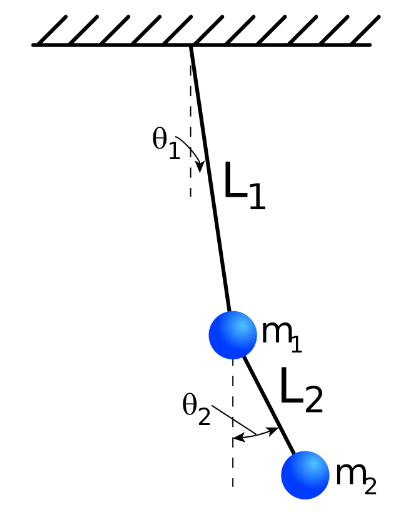
\includegraphics[width=2.5in]{dpend.png}
where an .eps filename suffix will be assumed under latex,
and a .pdf suffix will be assumed for pdflatex; or what has been declared
via \DeclareGraphicsExtensions.
\caption{Simulation Results}
\label{fig_sim}
\end{figure}

% Note that IEEE typically puts floats only at the top, even when this
% results in a large percentage of a column being occupied by floats.


% An example of a double column floating figure using two subfigures.
% (The subfig.sty package must be loaded for this to work.)
% The subfigure \label commands are set within each subfloat command, the
% \label for the overall figure must come after \caption.
% \hfil must be used as a separator to get equal spacing.
% The subfigure.sty package works much the same way, except \subfigure is
% used instead of \subfloat.
%
% \begin{figure*}[!t]
% \centerline{\subfloat[Case I]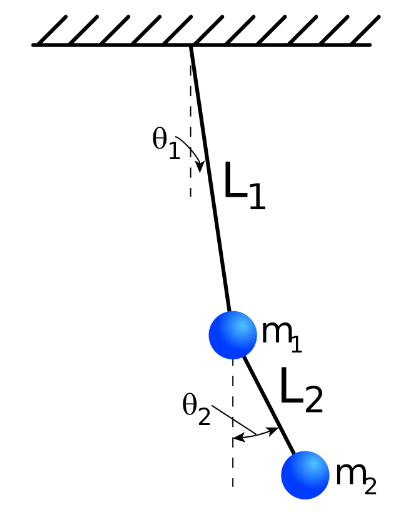
\includegraphics[width=2.5in]{dpend.png}%
% \label{fig_first_case}}
% \hfil
% \subfloat[Case II]{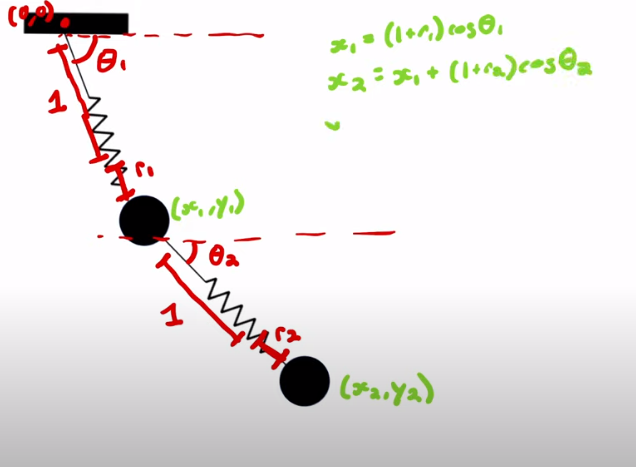
\includegraphics[width=2.5in]{dpend_sprg.png}%
% \label{fig_second_case}}}
% \caption{Simulation results}
% \label{fig_sim}
% \end{figure*}
%
% Note that often IEEE papers with subfigures do not employ subfigure
% captions (using the optional argument to \subfloat), but instead will
% reference/describe all of them (a), (b), etc., within the main caption.


% An example of a floating table. Note that, for IEEE style tables, the
% \caption command should come BEFORE the table. Table text will default to
% \footnotesize as IEEE normally uses this smaller font for tables.
% The \label must come after \caption as always.
%
%\begin{table}[!t]
%% increase table row spacing, adjust to taste
%\renewcommand{\arraystretch}{1.3}
% if using array.sty, it might be a good idea to tweak the value of
% \extrarowheight as needed to properly center the text within the cells
%\caption{An Example of a Table}
%\label{table_example}
%\centering
%% Some packages, such as MDW tools, offer better commands for making tables
%% than the plain LaTeX2e tabular which is used here.
%\begin{tabular}{|c||c|}
%\hline
%One & Two\\
%\hline
%Three & Four\\
%\hline
%\end{tabular}
%\end{table}


% Note that IEEE does not put floats in the very first column - or typically
% anywhere on the first page for that matter. Also, in-text middle ("here")
% positioning is not used. Most IEEE journals use top floats exclusively.
% Note that, LaTeX2e, unlike IEEE journals, places footnotes above bottom
% floats. This can be corrected via the \fnbelowfloat command of the
% stfloats package.



\section{Conclusion}
The conclusion goes here.







% \appendices
% \section{Proof of the First Zonklar Equation}
% Appendix one text goes here.

% you can choose not to have a title for an appendix
% if you want by leaving the argument blank
% \section{Appx B title}
% Appendix two text goes here.


% use section* for acknowledgement
\section*{Acknowledgment}
The authors would like to thank...


% Can use something like this to put references on a page
% by themselves when using endfloat and the captionsoff option.
% \ifCLASSOPTIONcaptionsoff
%   \newpage
% \fi

% trigger a \newpage just before the given reference
% number - used to balance the columns on the last page
% adjust value as needed - may need to be readjusted if
% the document is modified later
%\IEEEtriggeratref{8}
% The "triggered" command can be changed if desired:
%\IEEEtriggercmd{\enlargethispage{-5in}}

% references section

% can use a bibliography generated by BibTeX as a .bbl file
% BibTeX documentation can be easily obtained at:
% http://www.ctan.org/tex-archive/biblio/bibtex/contrib/doc/
% The IEEEtran BibTeX style support page is at:
% http://www.michaelshell.org/tex/ieeetran/bibtex/
%\bibliographystyle{IEEEtran}
% argument is your BibTeX string definitions and bibliography database(s)
%\bibliography{IEEEabrv,../bib/paper}
%
% <OR> manually copy in the resultant .bbl file
% set second argument of \begin to the number of references
% (used to reserve space for the reference number labels box)
\begin{thebibliography}{1}

\bibitem{IEEEhowto:kopka}
H.~Kopka and P.~W. Daly, \emph{A Guide to \LaTeX}, 3rd~ed.\hskip 1em plus
  0.5em minus 0.4em\relax Harlow, England: Addison-Wesley, 1999.

\end{thebibliography}

% biography section
%
% If you have an EPS/PDF photo (graphicx package needed) extra braces are
% needed around the contents of the optional argument to biography to prevent
% the LaTeX parser from getting confused when it sees the complicated
% \includegraphics command within an optional argument. (You could create
% your own custom macro containing the \includegraphics command to make things
% simpler here.)
%\begin{biography}[{\includegraphics[width=1in,height=1.25in,clip,keepaspectratio]{mshell}}]{Michael Shell}
% or if you just want to reserve a space for a photo:

% \begin{IEEEbiography}{Michael Shell}
% Biography text here.
% \end{IEEEbiography}

% % if you will not have a photo at all:
% \begin{IEEEbiographynophoto}{John Doe}
% Biography text here.
% \end{IEEEbiographynophoto}

% insert where needed to balance the two columns on the last page with
% biographies
%\newpage


% You can push biographies down or up by placing
% a \vfill before or after them. The appropriate
% use of \vfill depends on what kind of text is
% on the last page and whether or not the columns
% are being equalized.

%\vfill

% Can be used to pull up biographies so that the bottom of the last one
% is flush with the other column.
%\enlargethispage{-5in}



% that's all folks
\end{document}
